\pagenumbering{arabic}
\section{字母频率统计攻击方法}

\subsection{字母频率统计攻击方法流程}
\begin{figure}[thbp!]
	\centering
	
\includegraphics[width=16cm]{figure/figure3.png}
	\caption{字母频率统计攻击方法流程}
	\label{fig:字母频率统计攻击方法流程}
\end{figure}

\subsection{字母频率统计攻击方法程序代码}
\begin{lstlisting}[language=c++]
#include <iostream>
using namespace std;
int main()
{
	char* ciphertext = new char[1024];
	cin.getline(ciphertext, 1024);
	int len = strlen(ciphertext);
	
	//统计字母频率
	int num[26], total = 0;
	for (int i = 0; i < 26; i++)
	num[i] = 0;
	for (int i = 0; i < len; i++)
	{
		if (ciphertext[i] >= 'a' && ciphertext[i] <= 'z')
		{
			int n = ciphertext[i] - 'a';
			num[n]++;
			total++;
		}
		else if (ciphertext[i] >= 'A' && ciphertext[i] <= 'Z')
		{
			int n = ciphertext[i] - 'A';
			num[n]++;
			total++;
		}
	}
	
	int n[26][2];
	for (int i = 0; i < 26; i++)
	{
		n[i][0] = i;
		cout << char('a' + i) << "的频率为:" << float(num[i]) / total << endl;
	}
	
	//将字母按频率大小排序
	for (int i = 0; i < 26; i++)
	{
		for (int j = i; j < 26; j++)
		{
			if (num[i] < num[j])
			{
				swap(num[i], num[j]);
				int temp = n[i][0];
				n[i][0] = n[j][0];
				n[j][0] = temp;
			}
		}
	}
	//for (int i = 0; i < 26; i++)
	//{
		//    //cout << num[i] << endl;
		//    cout << char(n[i][0] + 'a') << endl;
		//}
	
	//创建n[26][2]二维数组,将排好序的字母与近似字母频率一一对应起来
	//其中n[i][0]储存排好序的字母,n[i][1]储存对应的近似字母
	//然后创建temp[26]创建置换表,将字母按顺序排好
	string str = "etoiansrhlducmpyfgwbvkxjqz";
	for (int i = 0; i < 26; i++)
	{
		n[i][1] = int(str[i] - 'a');
		//cout << n[i][1] << endl;
	}
	int temp[26];
	for (int i = 0; i < 26; i++)
	{
		temp[n[i][0]] = n[i][1];
	}
	
	//校正
	swap(temp['n' - 'a'], temp['j' - 'a']);
	swap(temp['y' - 'a'], temp['f' - 'a']);
	swap(temp['d' - 'a'], temp['x' - 'a']);
	swap(temp['m' - 'a'], temp['j' - 'a']);
	swap(temp['p' - 'a'], temp['r' - 'a']);
	swap(temp['q' - 'a'], temp['h' - 'a']);
	swap(temp['z' - 'a'], temp['a' - 'a']);
	swap(temp['e' - 'a'], temp['g' - 'a']);
	swap(temp['h' - 'a'], temp['x' - 'a']);
	swap(temp['a' - 'a'], temp['e' - 'a']);
	swap(temp['o' - 'a'], temp['k' - 'a']);
	
	cout << "置换表为:" << endl;
	for (int i = 0; i < 26; i++)
	{
		cout << char(i + 'a') << " ";
	}
	cout << endl;
	for (int i = 0; i < 26; i++)
	{
		cout << char(temp[i] + 'a') << " ";
	}
	cout << endl;
	
	for (int i = 0; i < len; i++)
	{
		if (ciphertext[i] >= 'A' && ciphertext[i] <= 'Z')
		ciphertext[i] = char(temp[ciphertext[i] - 'A'] + 'a');
		else if (ciphertext[i] >= 'a' && ciphertext[i] <= 'z')
		ciphertext[i] = char(temp[ciphertext[i] - 'a'] + 'a');
	}
	cout << ciphertext << endl;
	return 0;
}
\end{lstlisting}


\subsection{程序运行结果}
\begin{figure}[H]
	\centering
	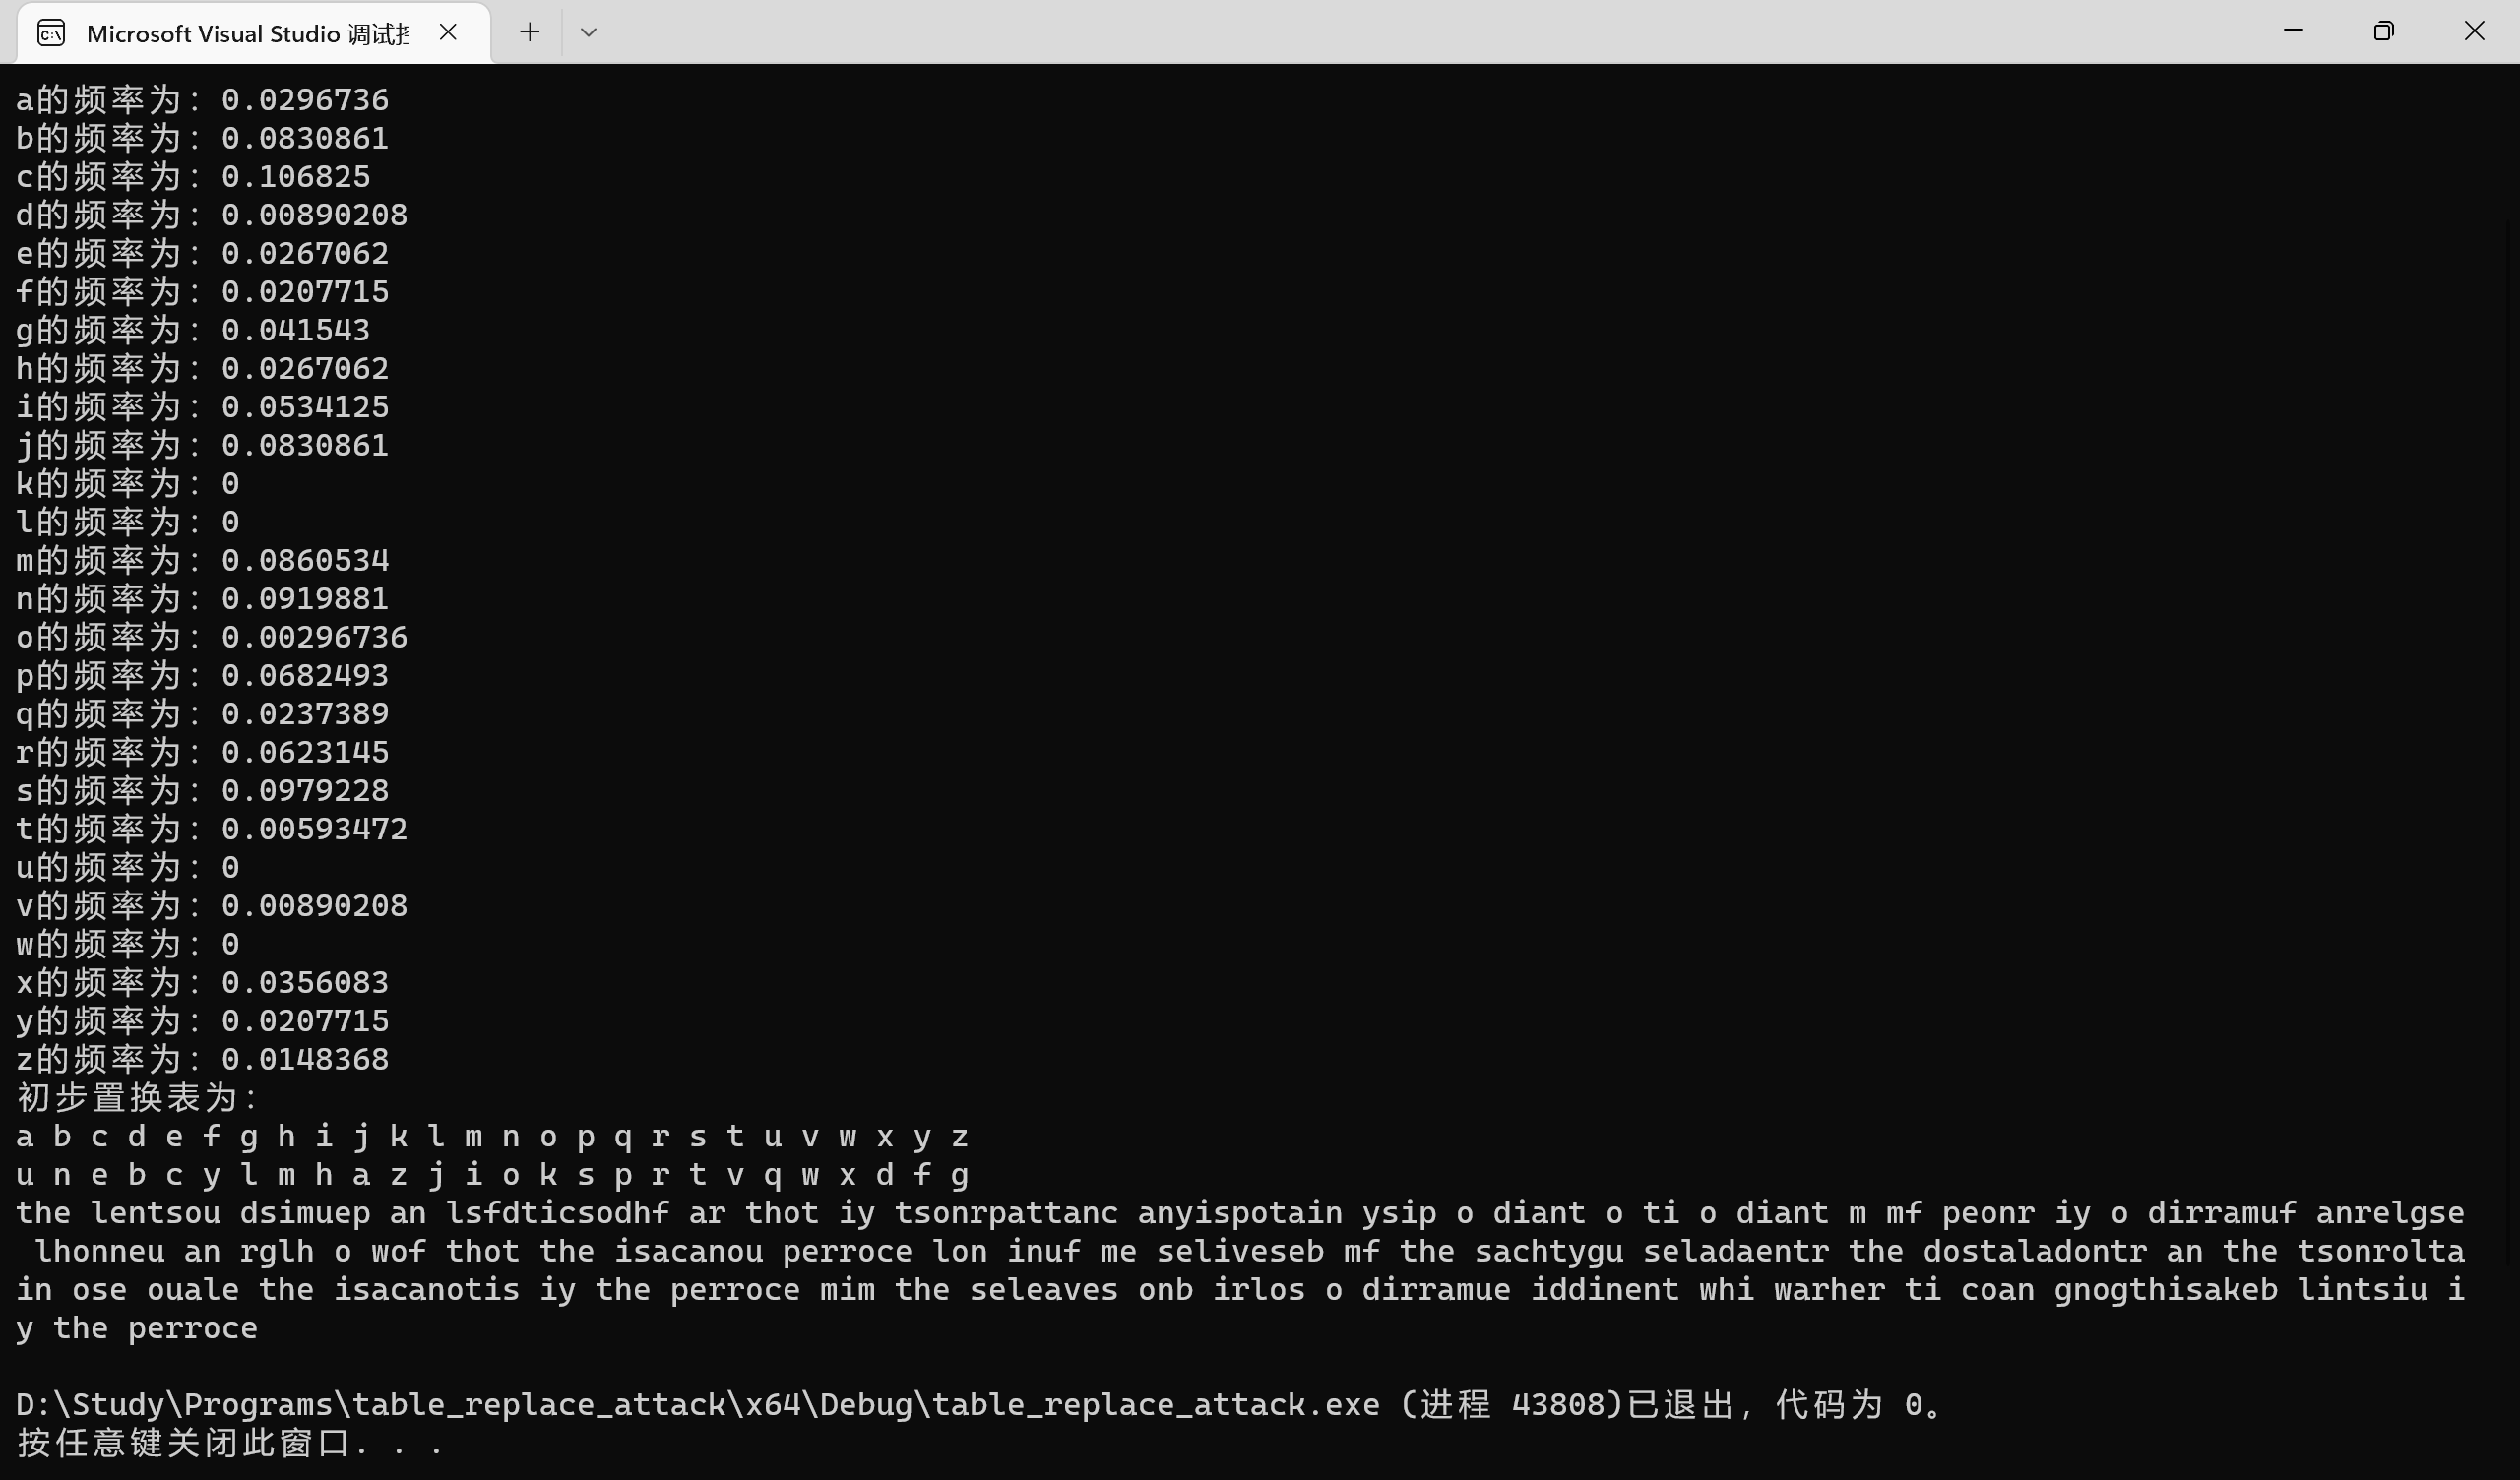
\includegraphics[width=16cm]{figure/004.png}
	\caption{字母频率统计攻击程序运行结果01}
	\label{fig:字母频率统计攻击程序运行结果01}
\end{figure}

\subsubsection{校正}
可以发现只依据单个字母的频率攻击得到的明文语义并不通顺,根据常用单词的频率

	将置换表中o、a互换\\
	置换表为:\\
	a b c d e f g h i j k l m n o p q r s t u v w x y z\\
	u n e b c y l m h o z j i a k s p r t v q w x d f g\\
	
	the lentsau dsimuep on lsfdticsadhf or that iy tsanrpottonc onyispatoin ysip a diont a ti a diont m mf peanr iy a dirromuf onrelgse lhanneu on rglh a waf that the isoconau perrace lan inuf me seliveseb mf the sochtygu selodoentr the dastolodantr on the tsanraltoin ase auole the isoconatis iy the perrace mim the seleoves anb irlas a dirromue iddinent whi worher ti caon gnagthisokeb lintsiu iy the perrace\\
	
	发现得到的明文中有"iy",应该是"if",将置换表中y、f互换\\
	
	置换表为:\\
	a b c d e f g h i j k l m n o p q r s t u v w x y z\\
	u n e b c f l m h o z j i a k s p r t v q w x d y g\\
	the lentsau dsimuep on lsydticsadhy or that if tsanrpottonc onfispatoin fsip a diont a ti a diont m my peanr if a dirromuy onrelgse lhanneu on rglh a way that the isoconau perrace lan inuy me seliveseb my the sochtfgu selodoentr the dastolodantr on the tsanraltoin ase auole the isoconatis if the perrace mim the seleoves anb irlas a dirromue iddinent whi worher ti caon gnagthisokeb lintsiu if the perrace\\
	
	发现得到的明文中有"anb",应该是"and",将置换表中b、d互换\\
	a b c d e f g h i j k l m n o p q r s t u v w x y z\\
	u n e d c f l m h o z j i a k s p r t v q w x b y g\\
	the lentsau bsimuep on lsybticsabhy or that if tsanrpottonc onfispatoin fsip a biont a ti a biont m my peanr if a birromuy onrelgse lhanneu on rglh a way that the isoconau perrace lan inuy me selivesed my the sochtfgu seloboentr the bastolobantr on the tsanraltoin ase auole the isoconatis if the perrace mim the seleoves and irlas a birromue ibbinent whi worher ti caon gnagthisoked lintsiu if the perrace\\
	
	发现得到的明文中有"ir",应该是"or",将置换表中i、o互换\\
	a b c d e f g h i j k l m n o p q r s t u v w x y z\\
	u n e d c f l m h i z j o a k s p r t v q w x b y g\\
	the lentsau bsomuep in lsybtocsabhy ir that of tsanrpittinc infospation fsop a boint a to a boint m my peanr of a borrimuy inrelgse lhanneu in rglh a way that the osicinau perrace lan onuy me selovesed my the sichtfgu selibientr the bastilibantr in the tsanraltion ase auile the osicinatos of the perrace mom the seleives and orlas a borrimue obbonent who wirher to cain gnagthosiked lontsou of the perrace\\
	
	发现得到的明文中有"frop",应该是"from",将置换表中p、m互换\\
	a b c d e f g h i j k l m n o p q r s t u v w x y z\\
	u n e d c f l p h i z j o a k r m s t v q w x b y g\\
	the lentrau bropuem in lrybtocrabhy is that of transmittinc information from a boint a to a boint p py means of a bossipuy inselgre lhanneu in sglh a way that the oricinau messace lan onuy pe relovered py the richtfgu relibients the bartilibants in the transaltion are auile the oricinator of the messace pop the releiver and oslar a bossipue obbonent who wishes to cain gnagthoriked lontrou of the messace\\
	
	
	发现得到的明文中有"py",应该是"by",将置换表中b、p互换\\
	a b c d e f g h i j k l m n o p q r s t u v w x y z\\
	g n e d l f c b h i z j o a k r m s t v q w x p y u\\
	the centrag probgem in cryptolraphy is that of transmittinl information from a point a to a point b by means of a possibgy insecure channeg in such a way that the orilinag messale can ongy be recovered by the rilhtfug recipients the participants in the transaction are agice the orilinator of the messale bob the receiver and oscar a possibge opponent who wishes to lain unauthoriked controg of the messale\\
	
	发现得到的明文中有"messale",应该是"message",将置换表中l、g互换\\
	a b c d e f g h i j k l m n o p q r s t u v w x y z\\
	l n e d g f c b h i z j o a k r m s t v q w x p y u\\
	the central problem in cryptography is that of transmitting information from a point a to a point b by means of a possibly insecure channel in such a way that the original message can only be recovered by the rightful recipients the participants in the transaction are alice the originator of the message bob the receiver and oscar a possible opponent who wishes to gain unauthoriked control of the message\\
	
	发现得到的明文中有"unauthoriked",应该是"unauthorized",将置换表中k、z互换,得到语义通顺的明文,攻击成功。\\
	置换表:\\
	a b c d e f g h i j k l m n o p q r s t u v w x y z\\
	l n e d g f c b h i k j o a z r m s t v q w x p y u\\
	the central problem in cryptography is that of transmitting information from a point a to a point b by means of a possibly insecure channel in such a way that the original message can only be recovered by the rightful recipients the participants in the transaction are alice the originator of the message bob the receiver and oscar a possible opponent who wishes to gain unauthorized control of the message\\



\begin{figure}[H]
	\centering
	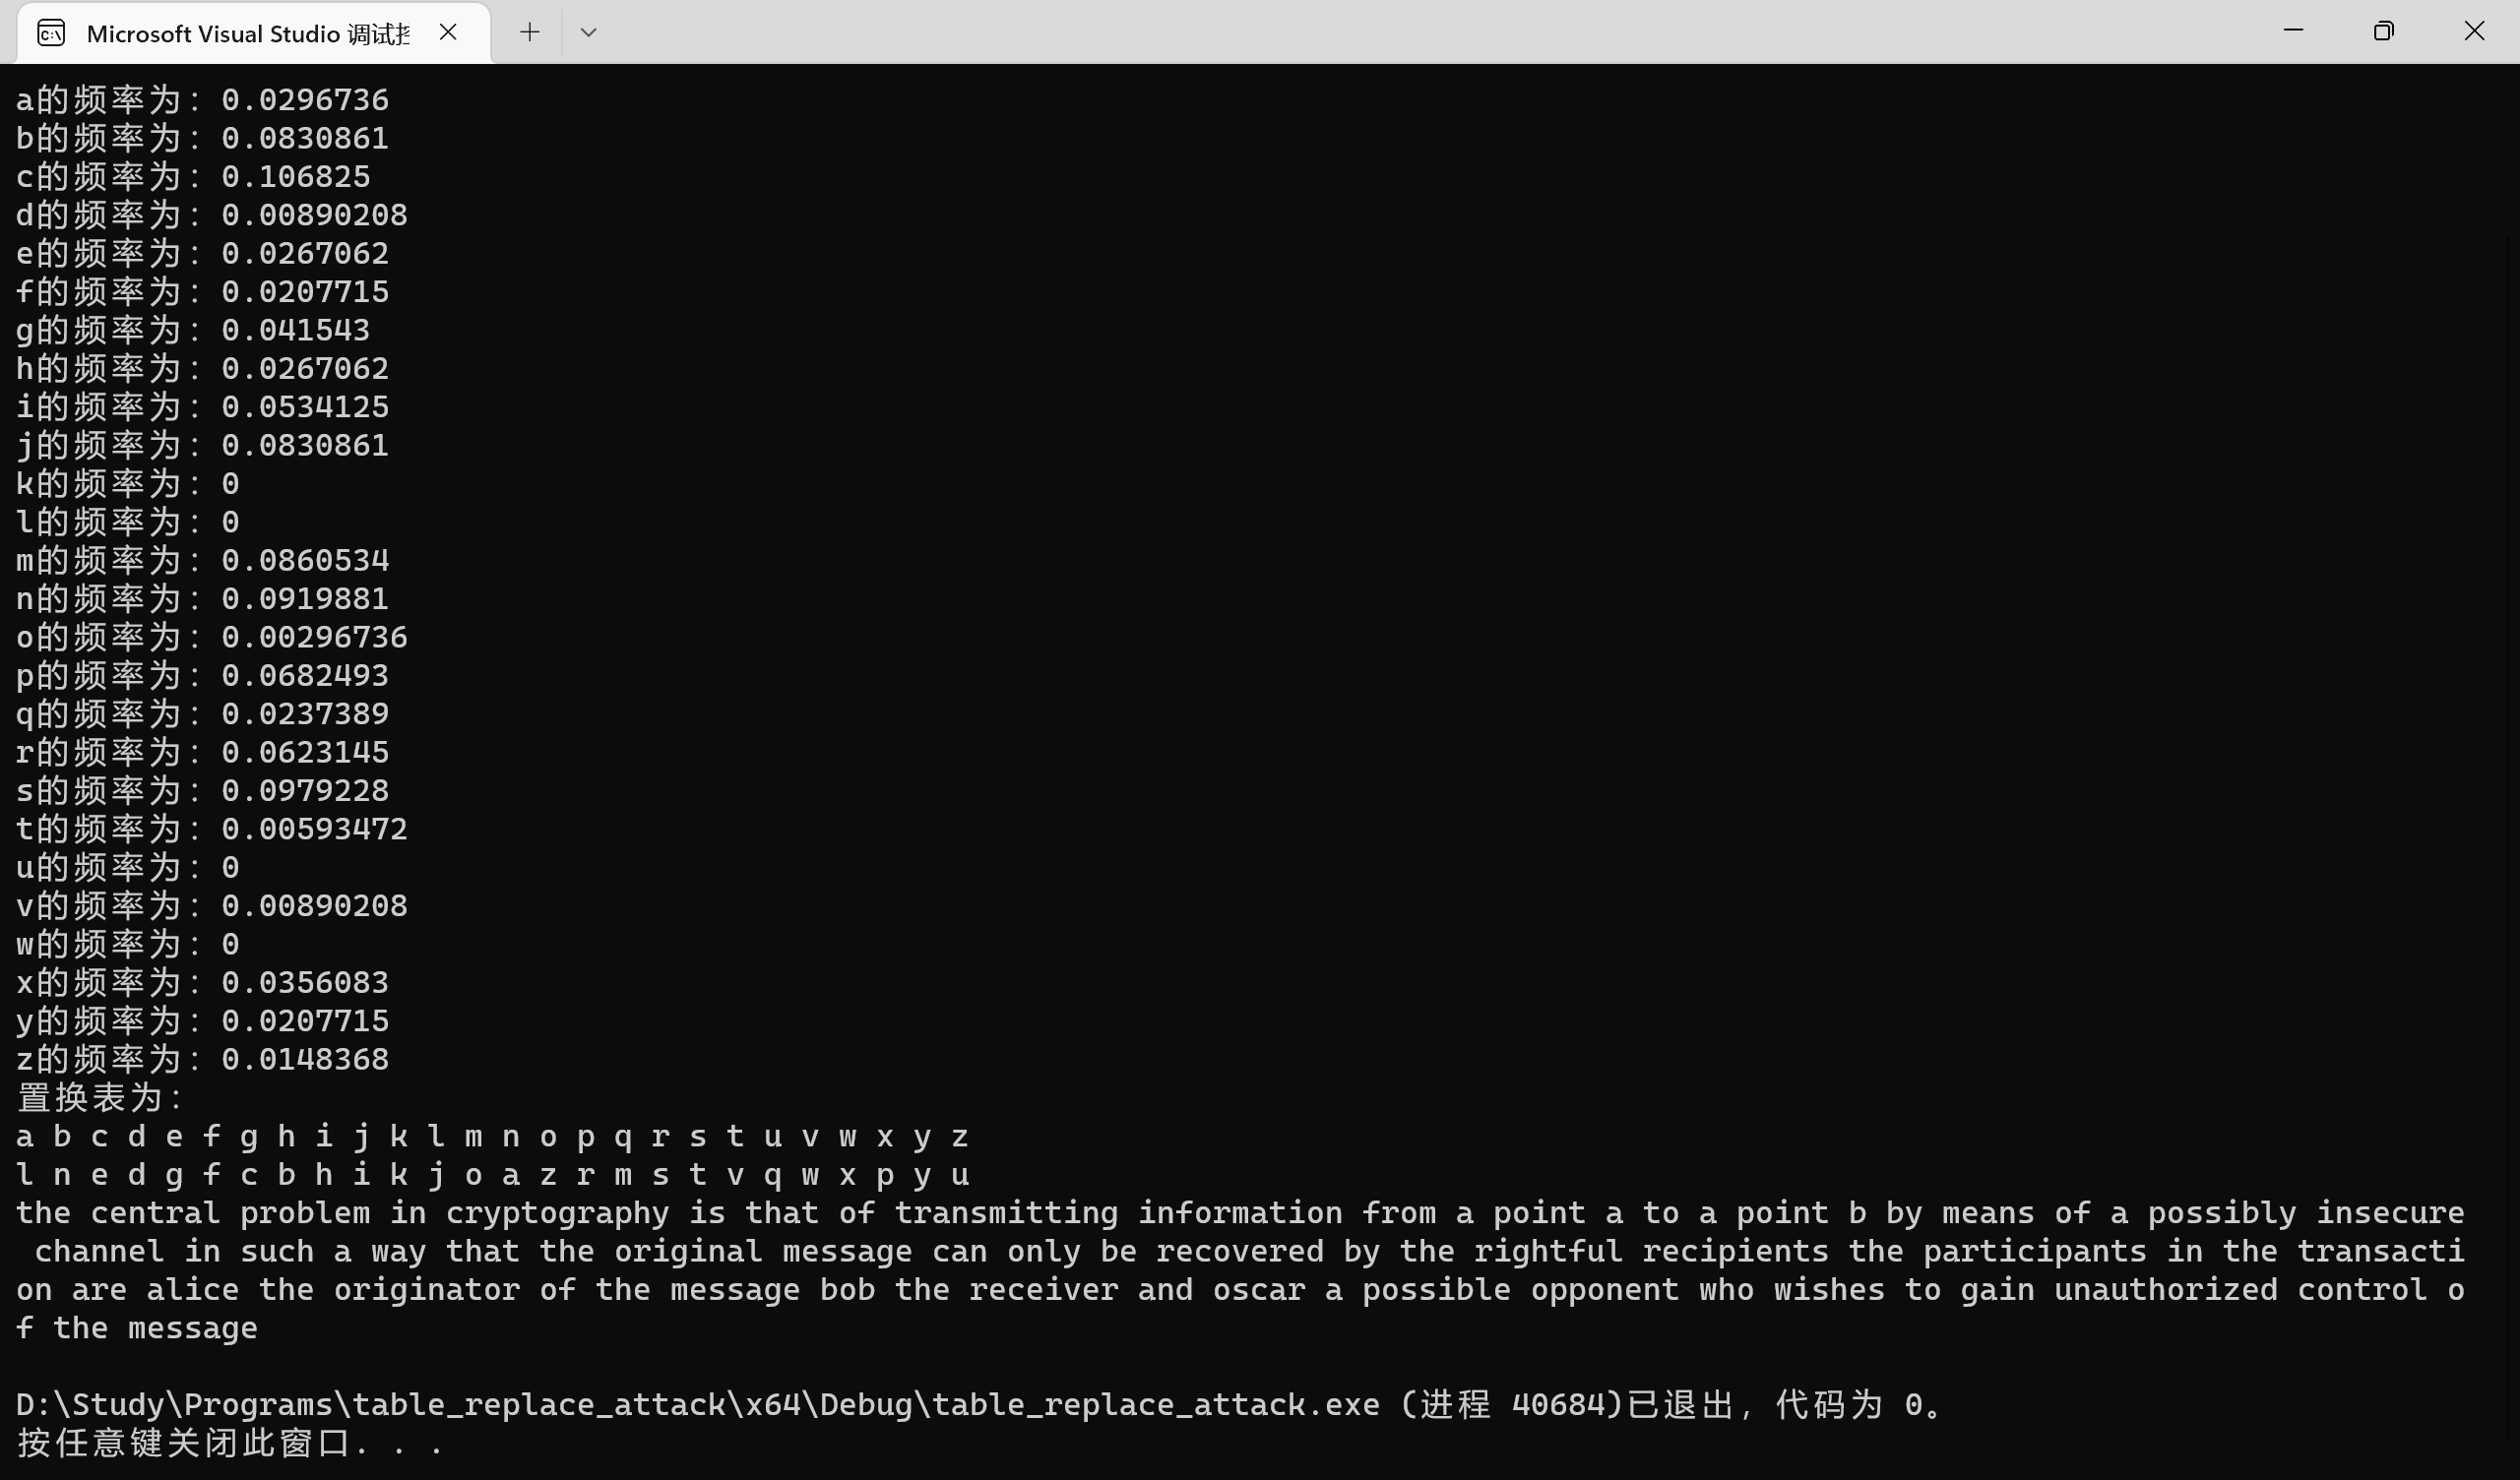
\includegraphics[width=16cm]{figure/005.png}
	\caption{字母频率统计攻击程序运行结果02}
	\label{fig:字母频率统计攻击程序运行结果02}
\end{figure}




